\documentclass[11pt]{article}
\usepackage{tikz}
\usetikzlibrary{positioning}

% Style matching the 2013 paper's tree drawings
\tikzset{
    % Root node with circled integer
    root/.style={
        draw, circle,
        minimum size=16pt,
        inner sep=1pt,
        font=\footnotesize
    },
    % Regular tree node (small hollow circle)
    tnode/.style={
        draw, circle,
        minimum size=5pt,
        inner sep=0pt,
        fill=white
    },
    % Edge style
    tedge/.style={
        thin
    },
    % Sibling and level distances for compact layout
    level 1/.style={sibling distance=12pt, level distance=10pt},
    level 2/.style={sibling distance=10pt, level distance=10pt},
    level 3/.style={sibling distance=8pt, level distance=10pt},
    level 4/.style={sibling distance=6pt, level distance=10pt},
}

% Command to draw a Matula tree
% Usage: \matulainteger{n}{tree structure}
\newcommand{\matulainteger}[2]{%
    \begin{tikzpicture}[baseline=(root.base)]
        \node[root] (root) {#1};
        #2
    \end{tikzpicture}%
}

% Shorthand for leaf (empty circle below parent)
\newcommand{\leaf}[1]{\node[tnode] (#1) {};}

\begin{document}

\section*{Integer-Tree Examples (Recreated Style)}

% Tree 1: single node
\matulainteger{1}{}

\bigskip

% Tree 2: root with one leaf
\matulainteger{2}{
    \node[tnode, below=8pt of root] (c1) {};
    \draw[tedge] (root) -- (c1);
}

\bigskip

% Tree 3: chain of depth 2
\matulainteger{3}{
    \node[tnode, below=8pt of root] (c1) {};
    \node[tnode, below=8pt of c1] (c2) {};
    \draw[tedge] (root) -- (c1) -- (c2);
}

\bigskip

% Tree 4: two leaves
\matulainteger{4}{
    \node[tnode, below left=8pt and 4pt of root] (c1) {};
    \node[tnode, below right=8pt and 4pt of root] (c2) {};
    \draw[tedge] (root) -- (c1);
    \draw[tedge] (root) -- (c2);
}

\bigskip

% Tree 5: chain of depth 3
\matulainteger{5}{
    \node[tnode, below=8pt of root] (c1) {};
    \node[tnode, below=8pt of c1] (c2) {};
    \node[tnode, below=8pt of c2] (c3) {};
    \draw[tedge] (root) -- (c1) -- (c2) -- (c3);
}

\bigskip

% Tree 6: one leaf + one chain
\matulainteger{6}{
    \node[tnode, below left=8pt and 4pt of root] (c1) {};
    \node[tnode, below right=8pt and 4pt of root] (c2) {};
    \node[tnode, below=8pt of c2] (c3) {};
    \draw[tedge] (root) -- (c1);
    \draw[tedge] (root) -- (c2) -- (c3);
}

\bigskip

% Tree 7: two children, one has two leaves
\matulainteger{7}{
    \node[tnode, below left=8pt and 6pt of root] (c1) {};
    \node[tnode, below right=8pt and 6pt of root] (c2) {};
    \node[tnode, below left=8pt and 3pt of c2] (c21) {};
    \node[tnode, below right=8pt and 3pt of c2] (c22) {};
    \draw[tedge] (root) -- (c1);
    \draw[tedge] (root) -- (c2);
    \draw[tedge] (c2) -- (c21);
    \draw[tedge] (c2) -- (c22);
}

\bigskip

% Tree 8: three leaves (star)
\matulainteger{8}{
    \node[tnode, below left=8pt and 6pt of root] (c1) {};
    \node[tnode, below=8pt of root] (c2) {};
    \node[tnode, below right=8pt and 6pt of root] (c3) {};
    \draw[tedge] (root) -- (c1);
    \draw[tedge] (root) -- (c2);
    \draw[tedge] (root) -- (c3);
}

\bigskip

% Tree 12: mix example (2*2*3 = p1*p1*p2)
\matulainteger{12}{
    \node[tnode, below left=8pt and 8pt of root] (c1) {};
    \node[tnode, below=8pt of root] (c2) {};
    \node[tnode, below right=8pt and 8pt of root] (c3) {};
    \node[tnode, below=8pt of c3] (c31) {};
    \draw[tedge] (root) -- (c1);
    \draw[tedge] (root) -- (c2);
    \draw[tedge] (root) -- (c3) -- (c31);
}

\bigskip

%% Grid layout example (like in the paper)
\section*{Grid of Trees 1--16}

\begin{center}
\begin{tabular}{cccccccc}
% Row 1: 1-8
\matulainteger{1}{} &
\matulainteger{2}{
    \node[tnode, below=6pt of root] (c1) {};
    \draw[tedge] (root) -- (c1);
} &
\matulainteger{3}{
    \node[tnode, below=6pt of root] (c1) {};
    \node[tnode, below=6pt of c1] (c2) {};
    \draw[tedge] (root) -- (c1) -- (c2);
} &
\matulainteger{4}{
    \node[tnode, below left=6pt and 3pt of root] (c1) {};
    \node[tnode, below right=6pt and 3pt of root] (c2) {};
    \draw[tedge] (root) -- (c1);
    \draw[tedge] (root) -- (c2);
} &
\matulainteger{5}{
    \node[tnode, below=6pt of root] (c1) {};
    \node[tnode, below=6pt of c1] (c2) {};
    \node[tnode, below=6pt of c2] (c3) {};
    \draw[tedge] (root) -- (c1) -- (c2) -- (c3);
} &
\matulainteger{6}{
    \node[tnode, below left=6pt and 3pt of root] (c1) {};
    \node[tnode, below right=6pt and 3pt of root] (c2) {};
    \node[tnode, below=6pt of c2] (c3) {};
    \draw[tedge] (root) -- (c1);
    \draw[tedge] (root) -- (c2) -- (c3);
} &
\matulainteger{7}{
    \node[tnode, below left=6pt and 5pt of root] (c1) {};
    \node[tnode, below right=6pt and 5pt of root] (c2) {};
    \node[tnode, below left=6pt and 2pt of c2] (c21) {};
    \node[tnode, below right=6pt and 2pt of c2] (c22) {};
    \draw[tedge] (root) -- (c1);
    \draw[tedge] (root) -- (c2);
    \draw[tedge] (c2) -- (c21);
    \draw[tedge] (c2) -- (c22);
} &
\matulainteger{8}{
    \node[tnode, below left=6pt and 5pt of root] (c1) {};
    \node[tnode, below=6pt of root] (c2) {};
    \node[tnode, below right=6pt and 5pt of root] (c3) {};
    \draw[tedge] (root) -- (c1);
    \draw[tedge] (root) -- (c2);
    \draw[tedge] (root) -- (c3);
}
\\[20pt]
% Row 2: 9-16 (simplified, would need full definitions)
9 & 10 & 11 & 12 & 13 & 14 & 15 & 16
\end{tabular}
\end{center}

\section*{The "86 Worked" Example}

% Recreating the worked example from page 5
\begin{center}
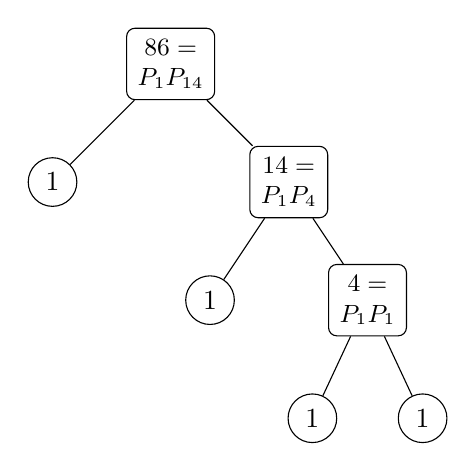
\begin{tikzpicture}[
    box/.style={draw, rounded corners=3pt, inner sep=4pt, align=center, font=\small},
    >=latex
]
    % Top node
    \node[box] (n86) at (0,0) {$86 =$ \\ $P_1 P_{14}$};

    % Left child (leaf = 1)
    \node[draw, circle, minimum size=14pt] (l1) at (-1.5,-1.5) {1};

    % Right child (14)
    \node[box] (n14) at (1.5,-1.5) {$14 =$ \\ $P_1 P_4$};

    % Children of 14
    \node[draw, circle, minimum size=14pt] (l2) at (0.5,-3) {1};
    \node[box] (n4) at (2.5,-3) {$4 =$ \\ $P_1 P_1$};

    % Children of 4
    \node[draw, circle, minimum size=14pt] (l3) at (1.8,-4.5) {1};
    \node[draw, circle, minimum size=14pt] (l4) at (3.2,-4.5) {1};

    % Edges
    \draw (n86) -- (l1);
    \draw (n86) -- (n14);
    \draw (n14) -- (l2);
    \draw (n14) -- (n4);
    \draw (n4) -- (l3);
    \draw (n4) -- (l4);
\end{tikzpicture}
\end{center}

\end{document}
